\documentclass[uplatex,dvipdfmx]{jsreport}

%\usepackage{luatexja}
\usepackage{docmute}

%\usepackage[2.0]{bxpdfver}


\usepackage{graphicx}

\usepackage{xcolor}
\graphicspath{{./docs/images/}{./images/}}
\definecolor{forground}{gray}{0.75}
\definecolor{background}{gray}{0.10}
\color{forground}
\pagecolor{background}

\usepackage{siunitx}

\usepackage{tikz}
\usetikzlibrary{intersections,calc,arrows.meta}

%\usepackage[style=base]{caption}
\usepackage[subrefformat=parens]{subcaption}

\usepackage{prettyref}
\newrefformat{note}{脚注~\ref*{#1}}
\newrefformat{figs}{図~\ref*{#1}}
\newrefformat{fig}{図~\ref*{#1}}
\newrefformat{tbl}{表~\ref*{#1}}
\newcommand*{\fullref}[1]{\hyperref[#1]{\prettyref{#1}}}

\usepackage[pdfusetitle,hidelinks]{hyperref}
\usepackage{pxjahyper}

\newcommand*{\includefig}[5][c]{%
    \begin{minipage}[#1]{#2\linewidth}
        \centering
        \includegraphics[width=\linewidth]{#5}
        \subcaption{#3}
        \label{#4}
    \end{minipage}
}
\newenvironment{imageHere}[2][htbp]{\def\@imageHereTmp{#2}%
    \begin{figure}[#1]
        \centering
}{%  
        \caption{\@imageHereTmp}
        \label{figs:\@imageHereTmp}
    \end{figure}
}

\title{
    コズミックトラベル (編集中) \\
    \large 75th2600内装設計チーフ引き継ぎ
}
\author{75th621 千葉森生}
\date{最終更新日: \today}

\begin{document}

\section{概要}
\subsection{成果物}

まずは作ったものの紹介から。

\begin{imageHere}{骨組み}
    \includefig{0.45}{完成形}{fig:完成形}{plan_overview/2.jpg}
    \includefig{0.45}{完成直前}{fig:完成直前}{plan_overview/3.jpg}
\end{imageHere}

正三角形のパーツを6個作り、ネジで繋ぎ合わせて作りました。後述しますが、分割して組み立てる方法は教室復元\footnote{\hyperlink{note:教室復元}{p.7の脚注}を参照}を意識したものなので、似たようなのを作る場合は分割せずまとめて作ってしまうのもありかと思います。
特徴としては、稼働部が巨大であること、それに応じて補強も複雑であることです。


\begin{imageHere}{装飾後}
    \begin{minipage}{0.45\linewidth}
        \centering
        \includefig{1}{宇宙船の内装}{fig:内装}{plan_overview/4.jpg}
        \includefig{1}{降りた後の通路から出口方面}{fig:出口}{plan_overview/5.jpg}
    \end{minipage}\hfill
    \begin{minipage}{0.45\linewidth}
        \centering
        \includefig{1}{ライドを動かす様子}{fig:人力}{plan_overview/6.jpg}
    \end{minipage}
\end{imageHere}

基本的に二人乗りですが、動き回ることを想定しているので実際は5人ぐらい入っても問題ない大きさ。もっとも、ライドを回すのは人力なので、あまり重いと回りませんが。

\clearpage

\subsection{動線}

\begin{imageHere}{動線}
    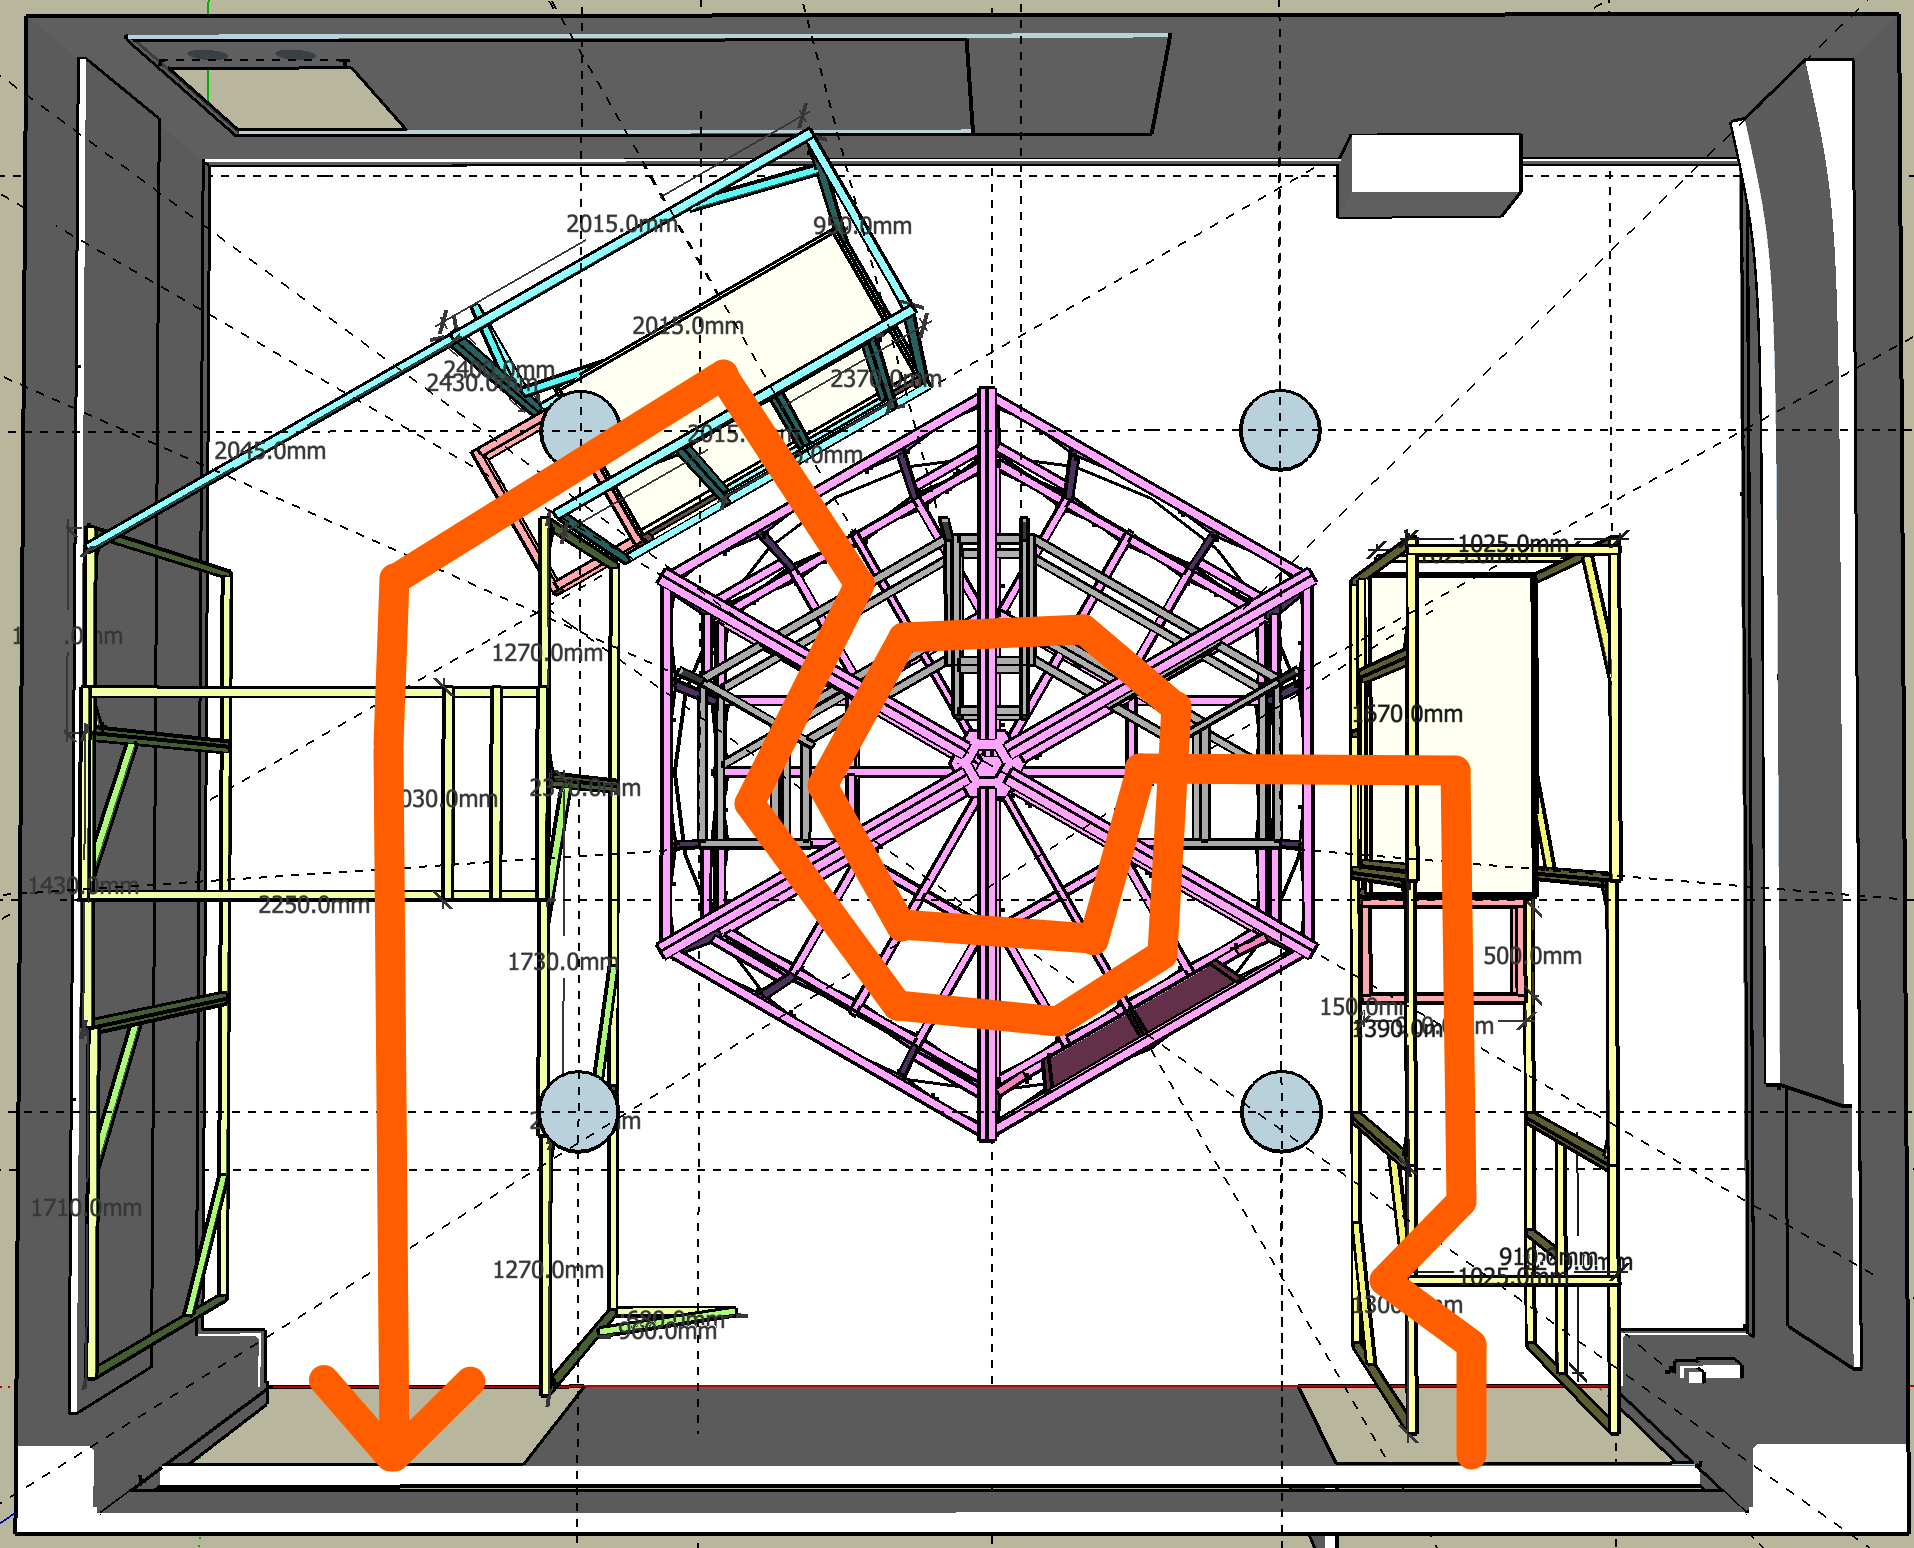
\includegraphics[width=0.6\linewidth]{plan_overview/lane.png}
\end{imageHere}

\begin{enumerate}
    \item 教室前方のドアが入り口、入って左側に受付
    \item そのまま進み、渡し板を渡って宇宙船に乗り込む
    \item ミニゲームを解く間に、ストーリーに合わせて宇宙船が回転
    \item 宇宙船から降りた後、出口側の通路でミニゲームの結果に応じた映像を流す
    \item 教室後方から出て終了
\end{enumerate}

\end{document}